\section{Experimenting with Reaching}\label{sec:reach-no-obs}

\subsection{Creating a Policy}
I am mainly working on imitation learning -and specifically behavioural cloning- from demonstrations provided by the system. A network needs to be able to ingest these demonstrations and generate actions in the action space of the robot. I created the following network, Figure \ref{fig:policy-arch}. This takes in the given wrist rgb image and extracts features, which are then interpreted into a $8$ dim vector of \textbf{float}s as an action of joint velocities. First $7$ corresponding to the $7$ joints of the \emph{Panda} robot, while the final value is the gripper state, $0$ meaning closed and $1$ meaning open, which is clamped by the movement system under the hood.

\subsubsection{Data Processing}\todo[color=red]{talk about rgb transforms? uniforming etc, or not not sure}
How the data is regularised, processed, and loaded into the system for training or testing is quite important for any Machine Learning (ML) task. The main processing I applied to the data was normalisation and scaling. RLBench, by default, returns image colour values in the range \(\left[0, 255\right]\) which was transformed to be in range \(\left[0.0, 1.0\right]\). Done before both inference and training. Mainly to keep weight magnitudes manageable for faster convergence, due to optimisers and activation functions working better at smaller scales. Secondly, this means that each pixel in the image will contribute to the extruded feature proportionally. Without the use of raw, meaningless numbers. This will help the numerical stability of the task.

\subsubsection{Data Loading}\label{subsec:reach-data-loading}
I followed a simple flattening approach for loading the data into the system. Using PyTorch's \textbf{Dataset} and \textbf{DataLoader} classes I created a dataset that can take in a raw list of demonstration, then flattens its observations into a tensor of shape \(\langle 3,~64,~64 \rangle \) (permuted from the usual \(\langle 64,~64,~3 \rangle \) for images due to Torch conventions of convolutional networks and where they expect the channel  dimension). Then the dataset makes individual observation indexable along with their corresponding action labels. Types given as:\mintinline{python}|DemoObsDataset: tuple[tensor[3,  64, 64], tensor[8]]|. Then the loader can manage the shuffling and batching as usual. Initially I kept the data unshuffled, to keep the data in its sequential form.

\subsection{Initial Observations}
Starting with the 3 static versions of the task, where the target is placed as shown in \ref{fig:no-obs-3-views} seen from the wrist cameras. I wanted to get an idea of how to tune the policy parameters. While understanding the relationship between training length and varying observability of the target.

\begin{figure}[htbp]
  \begin{subfigure}{0.3\linewidth}
    \centering
    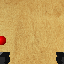
\includegraphics[width=0.6\linewidth]{assets/cam-comb/reach-no-obs/initial-obs-side_l.png}      
    \caption{Left Side}
  \end{subfigure}
  \hfill
  \begin{subfigure}{0.3\textwidth}
    \centering
    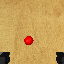
\includegraphics[width=0.6\linewidth]{assets/cam-comb/reach-no-obs/initial-obs-central.png}
    \caption{Central}
  \end{subfigure}
  \hfill
  \begin{subfigure}{0.3\textwidth}
    \centering 
    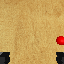
\includegraphics[width=0.6\linewidth]{assets/cam-comb/reach-no-obs/initial-obs-side_r.png}
    \caption{Right Side}
  \end{subfigure}%
  \caption{Three variations of the reach task with the obstacles sometimes out of view}\label{fig:no-obs-3-views}
\end{figure}

I tested multiple epochs of training with the simple policy and recorded the final distance to the target at the end of their episode. The episode length is determined by the demo lengths, which I defaulted to the maximum, will also try mean, as keeping a static episode length doesn't make sense (especially on later tasks where the demonstration episodes can drastically vary in length)

The success of the tasks are wired to reaching the target in the simulator and will send a \emph{DONE} signal if it is reached. This happens around $0.12$ metres to the target. I have also observed the target will reach a very close distance but it won't trigger the detection in Coppelia, I think this must be a bounding box issue, wither the dummy objects that are doing the collision detection are missing each other, or the polling rate in the simulator is not frequent enough to detect this change. Either way, I added a way to count closeness into success if it were close enough.

\subsubsection{Static Tasks}
Testing on the static versions of the task, a simple policy with training around $20$ to $100$ epochs seems to do the job well, see Figure \ref{subfig:rno-static}. And this is mostly because without variation in position simple Behavioural Cloning can be employed by overfitting to the data given. Overtraining meant actions got stuck at the top, wasting steps and ending up far from the target. Curious observation is \todo[color=purple]{} the central tasks behaves better at higher epochs which I believe is not necessarily because of visibility but rather the centrality, as it is right above the gripper a simple downward bias allows the arm to easily get close to the target.

\subsubsection{Placing Randomly}
To test generalisability, I created a dynamic version of the task, where the target is now randomly placed within view (not always fully within view). This is achieved by using a \textbf{SpawnBoundary} and randomly sampling the location of the target withing this for every new variation of the task, or for every new episode. Which can be seen in Figure \ref{fig:reach-no-obs}, the white dotted box being the boundary. This boundary is not rendered in the simulation visually. This guarantees variety in demonstrations as well as helps us create a generalisable policy.

\begin{figure}[htpb] % htpb allows all placement
  \begin{subfigure}{0.3\linewidth}
    \centering
    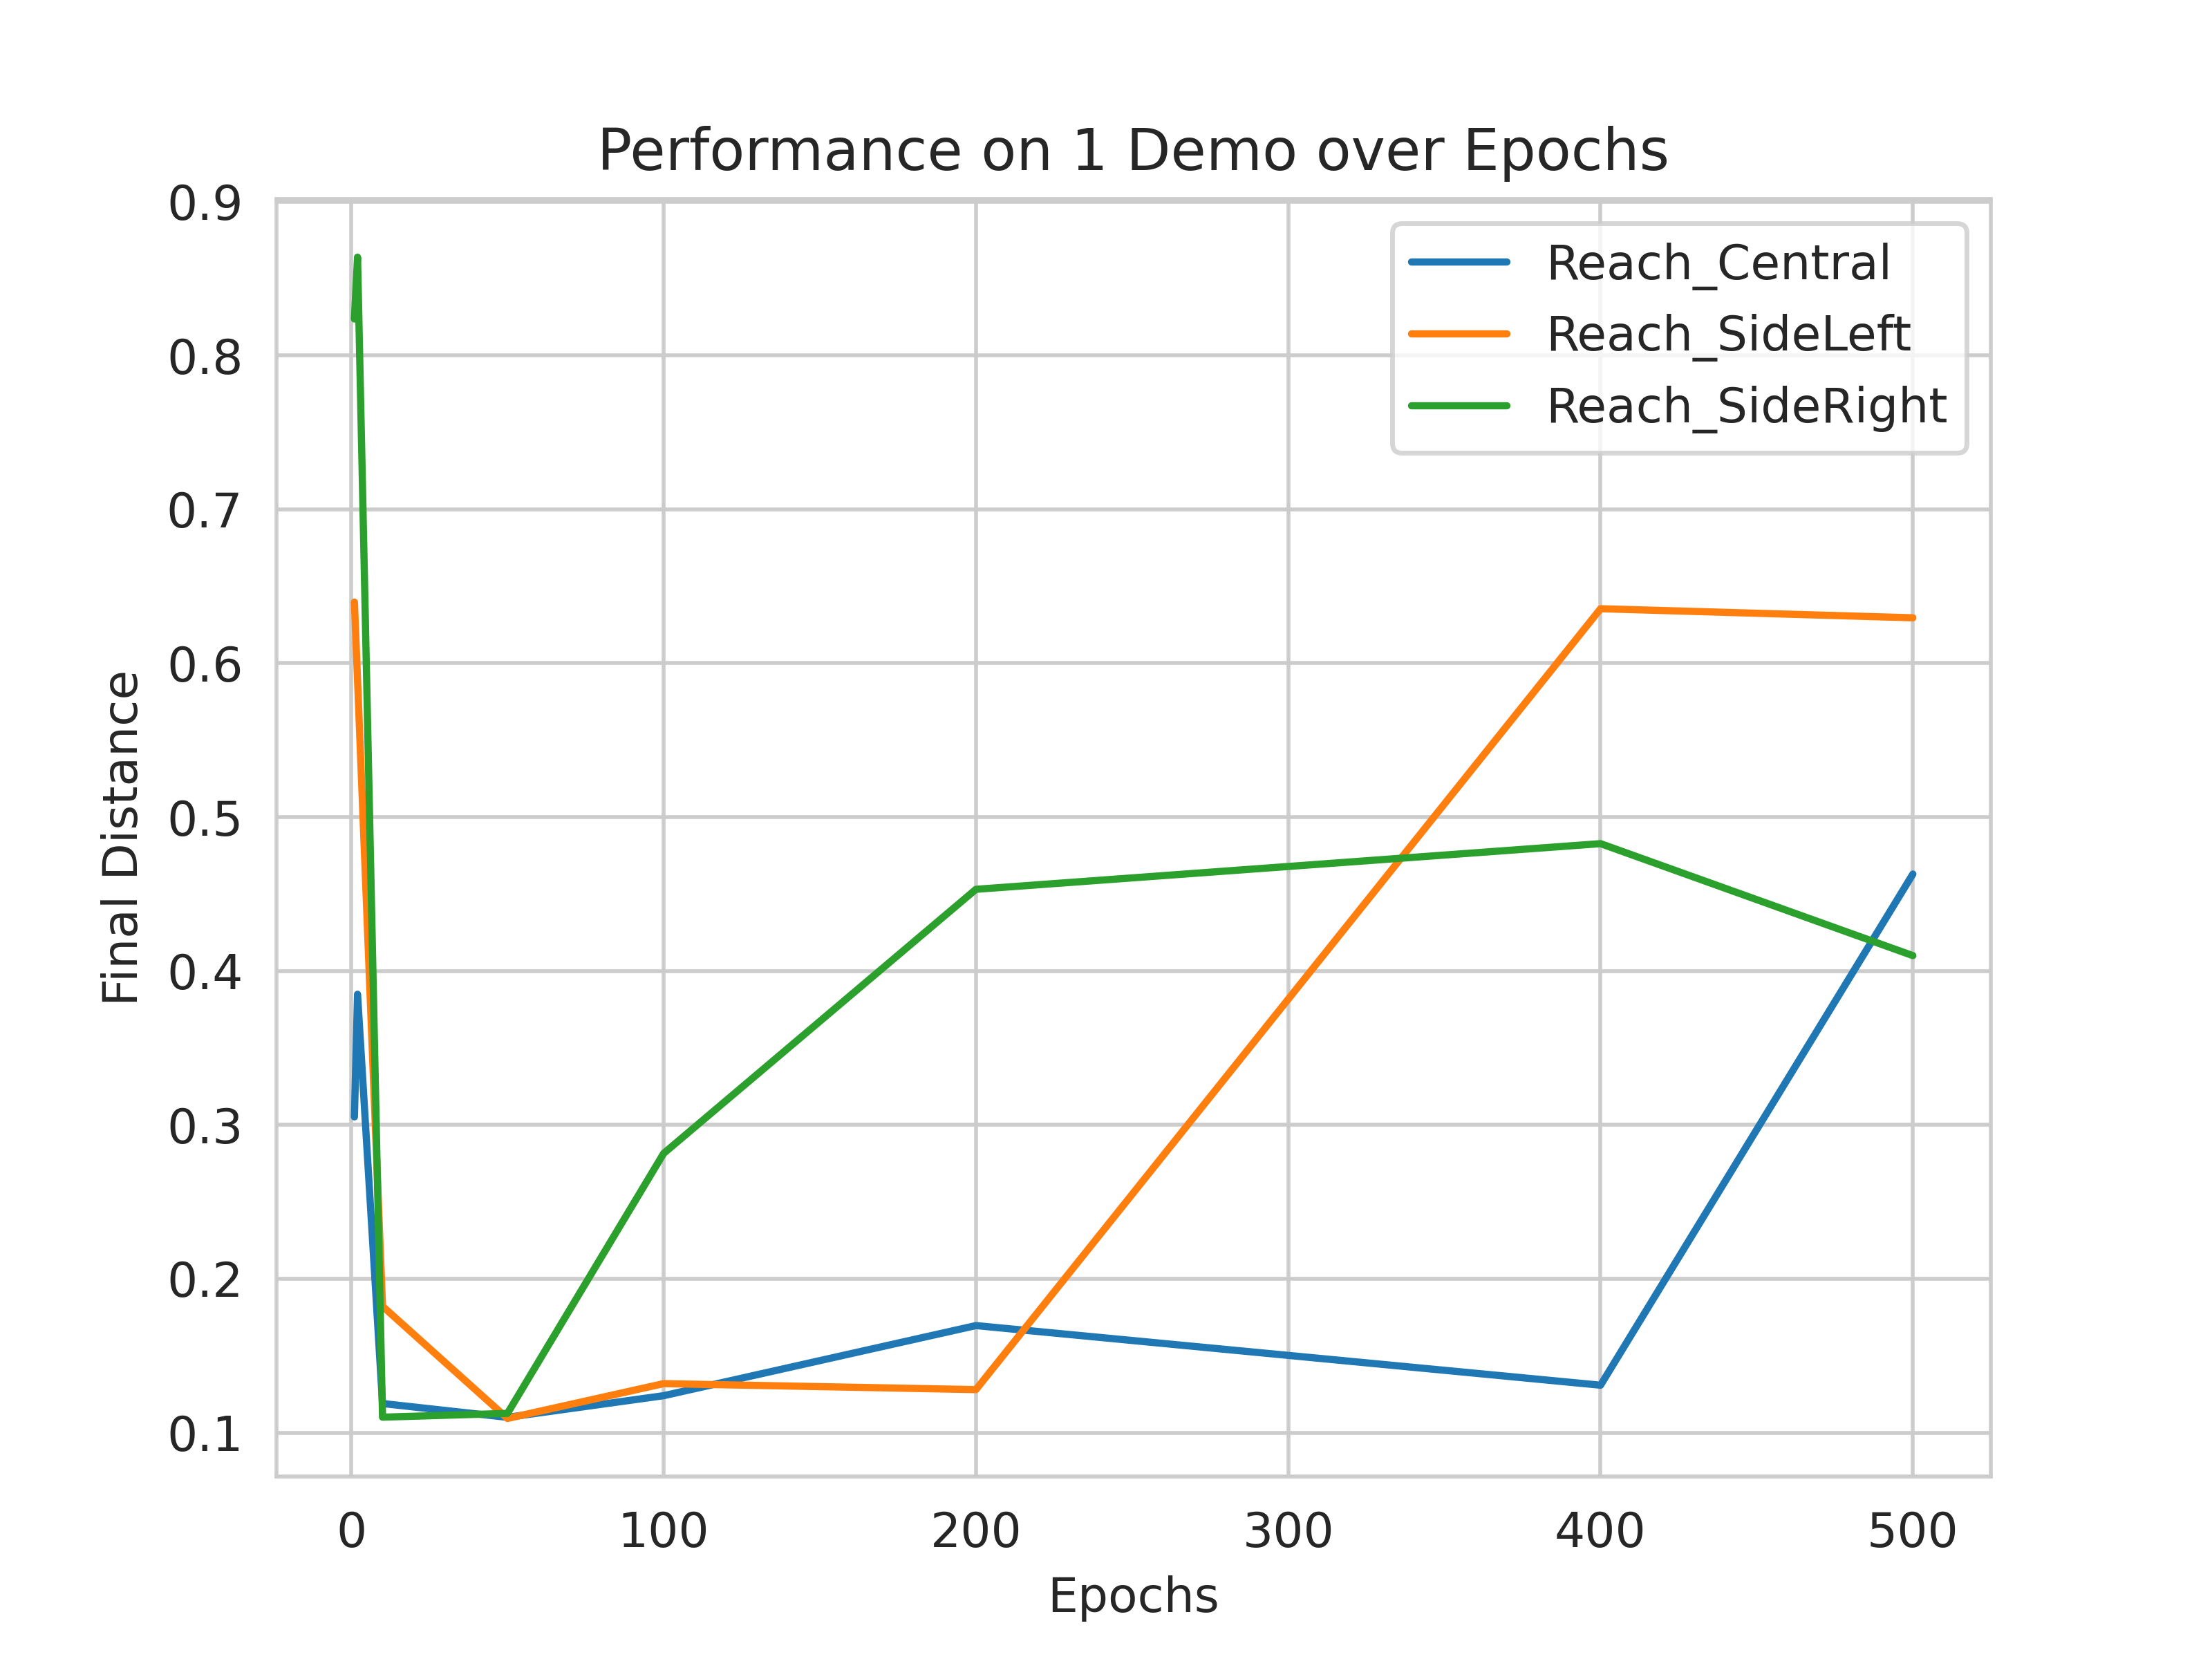
\includegraphics[width=\linewidth]{assets/cam-comb/reach-no-obs/rno_static.png}
    \caption{Static experiments with a single demo}\label{subfig:rno-static}
  \end{subfigure}
  \begin{subfigure}{0.3\linewidth}
    \centering
    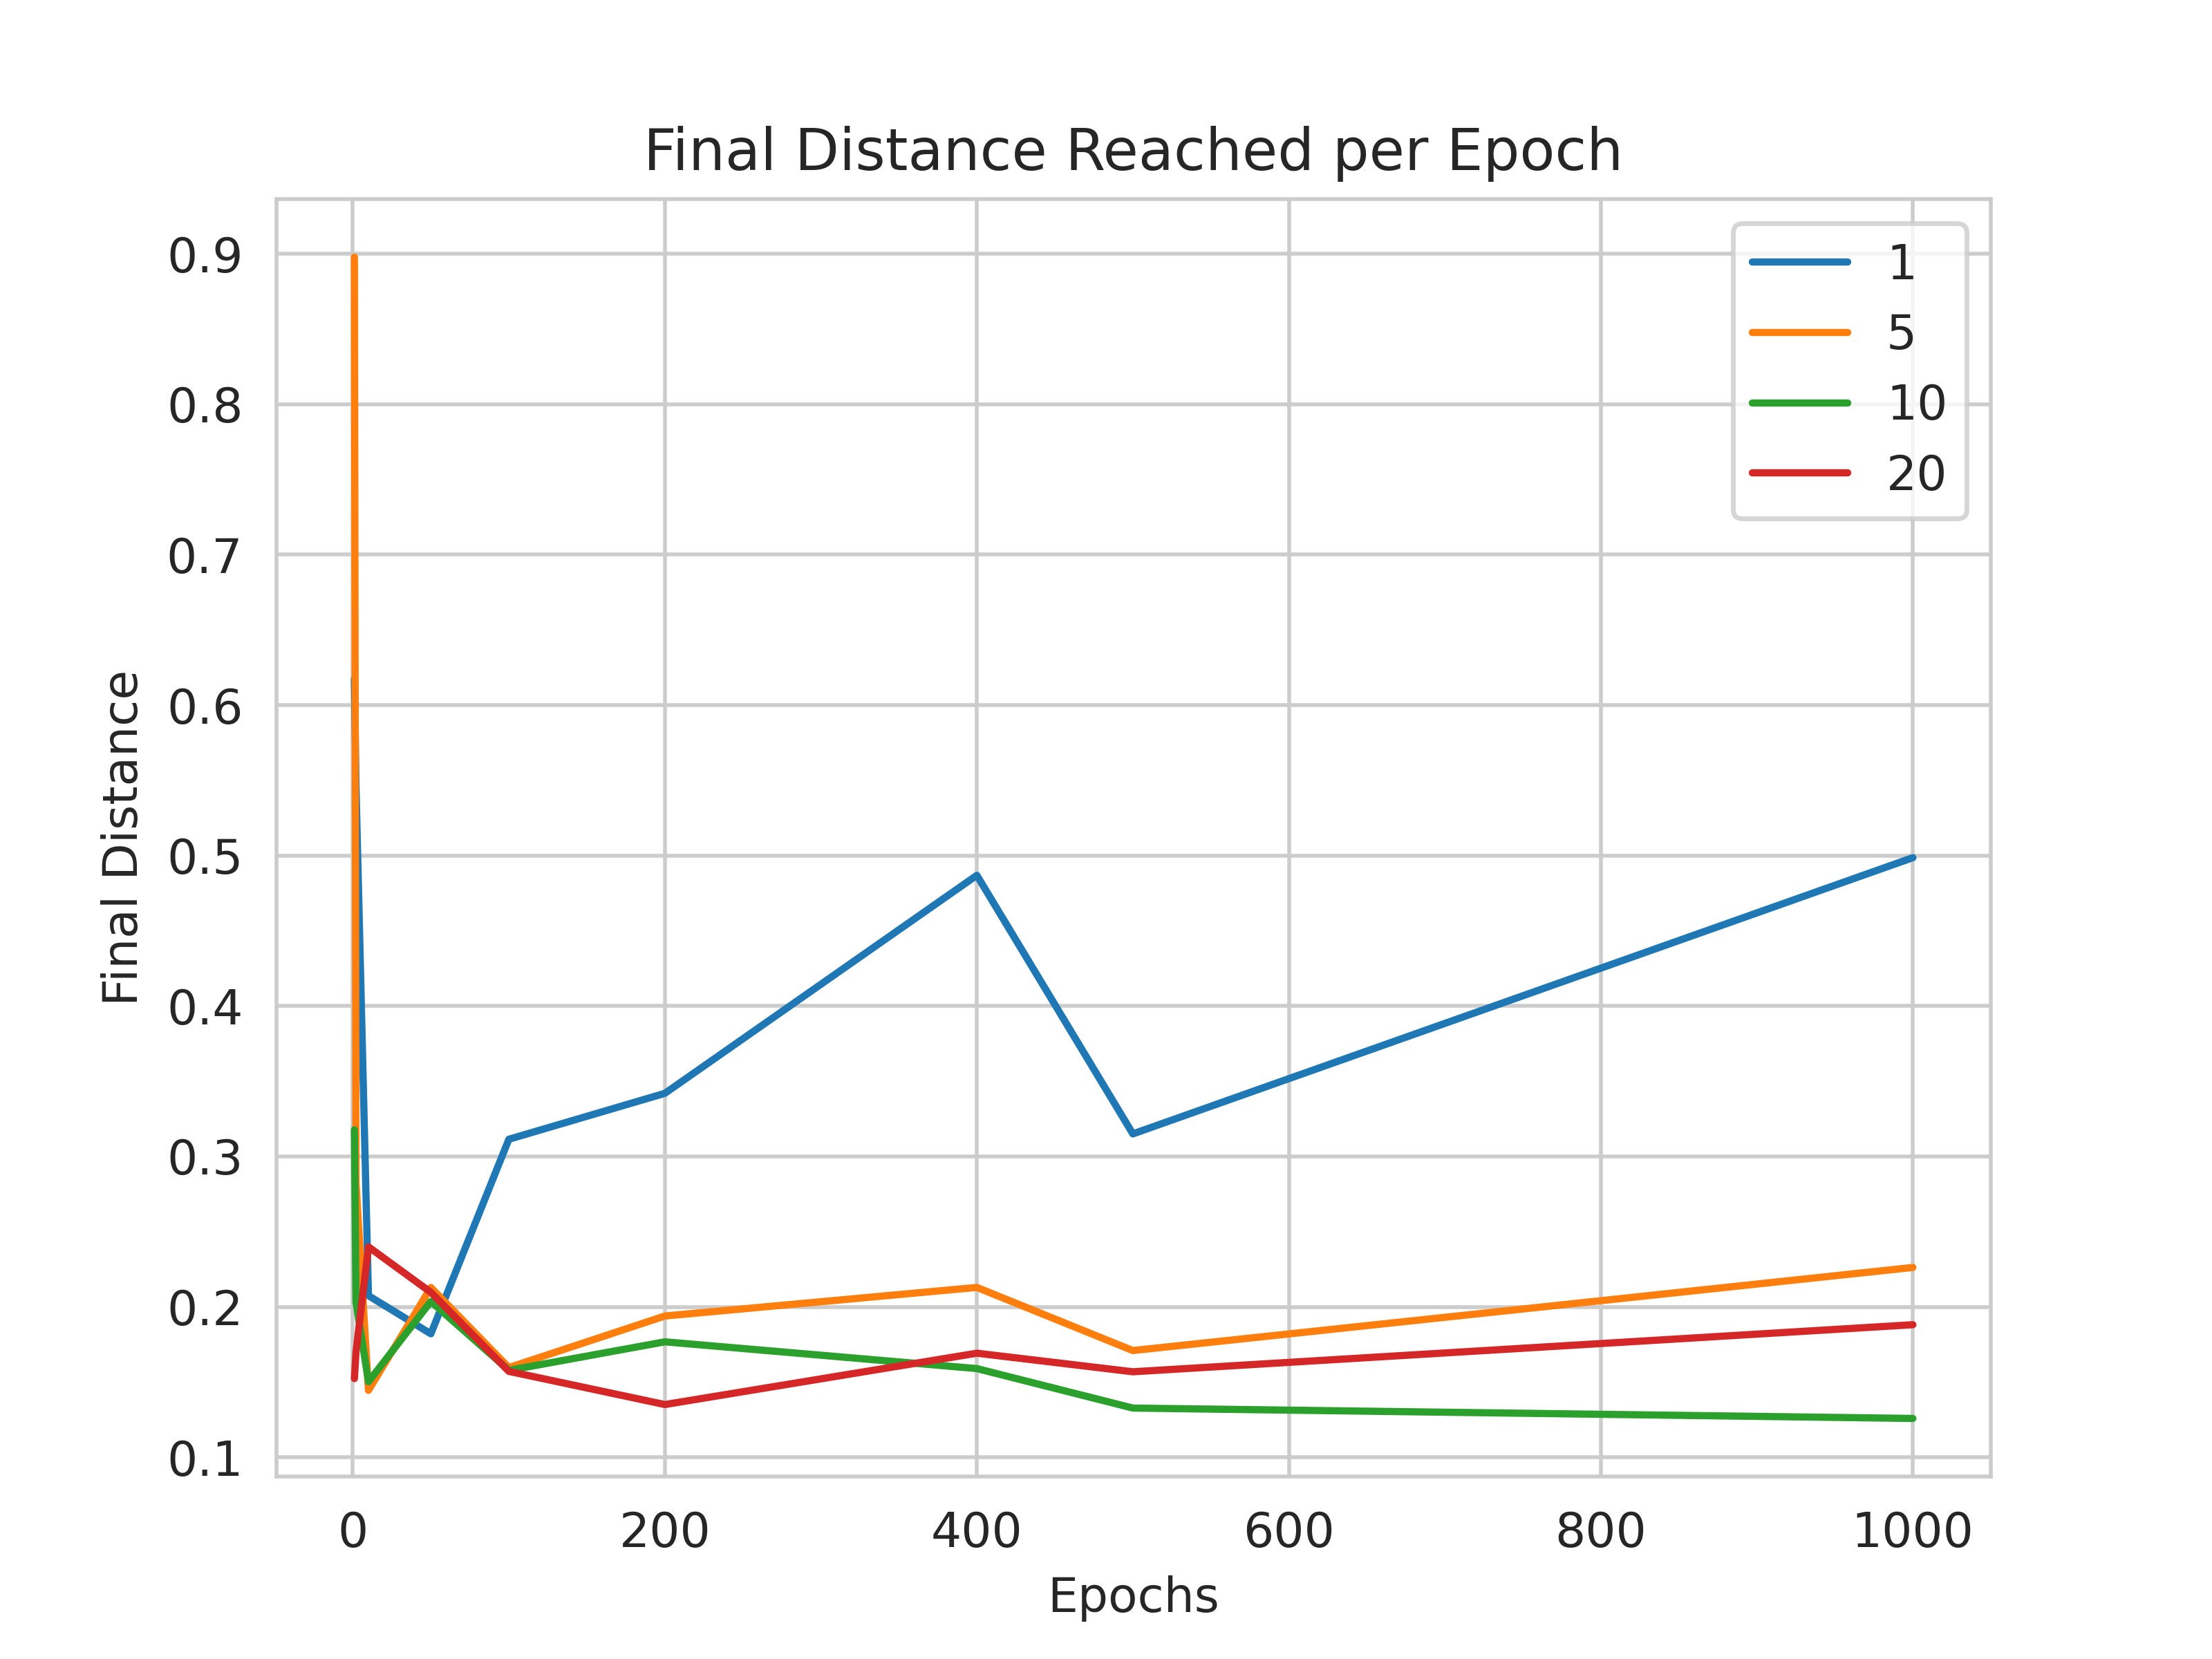
\includegraphics[width=\linewidth]{assets/cam-comb/reach-no-obs/rno_random-dist.png}
    \caption{Average Final Distance to Target}\label{subfig:rno-random-dist}
  \end{subfigure}
  \begin{subfigure}{0.3\linewidth}
    \centering
    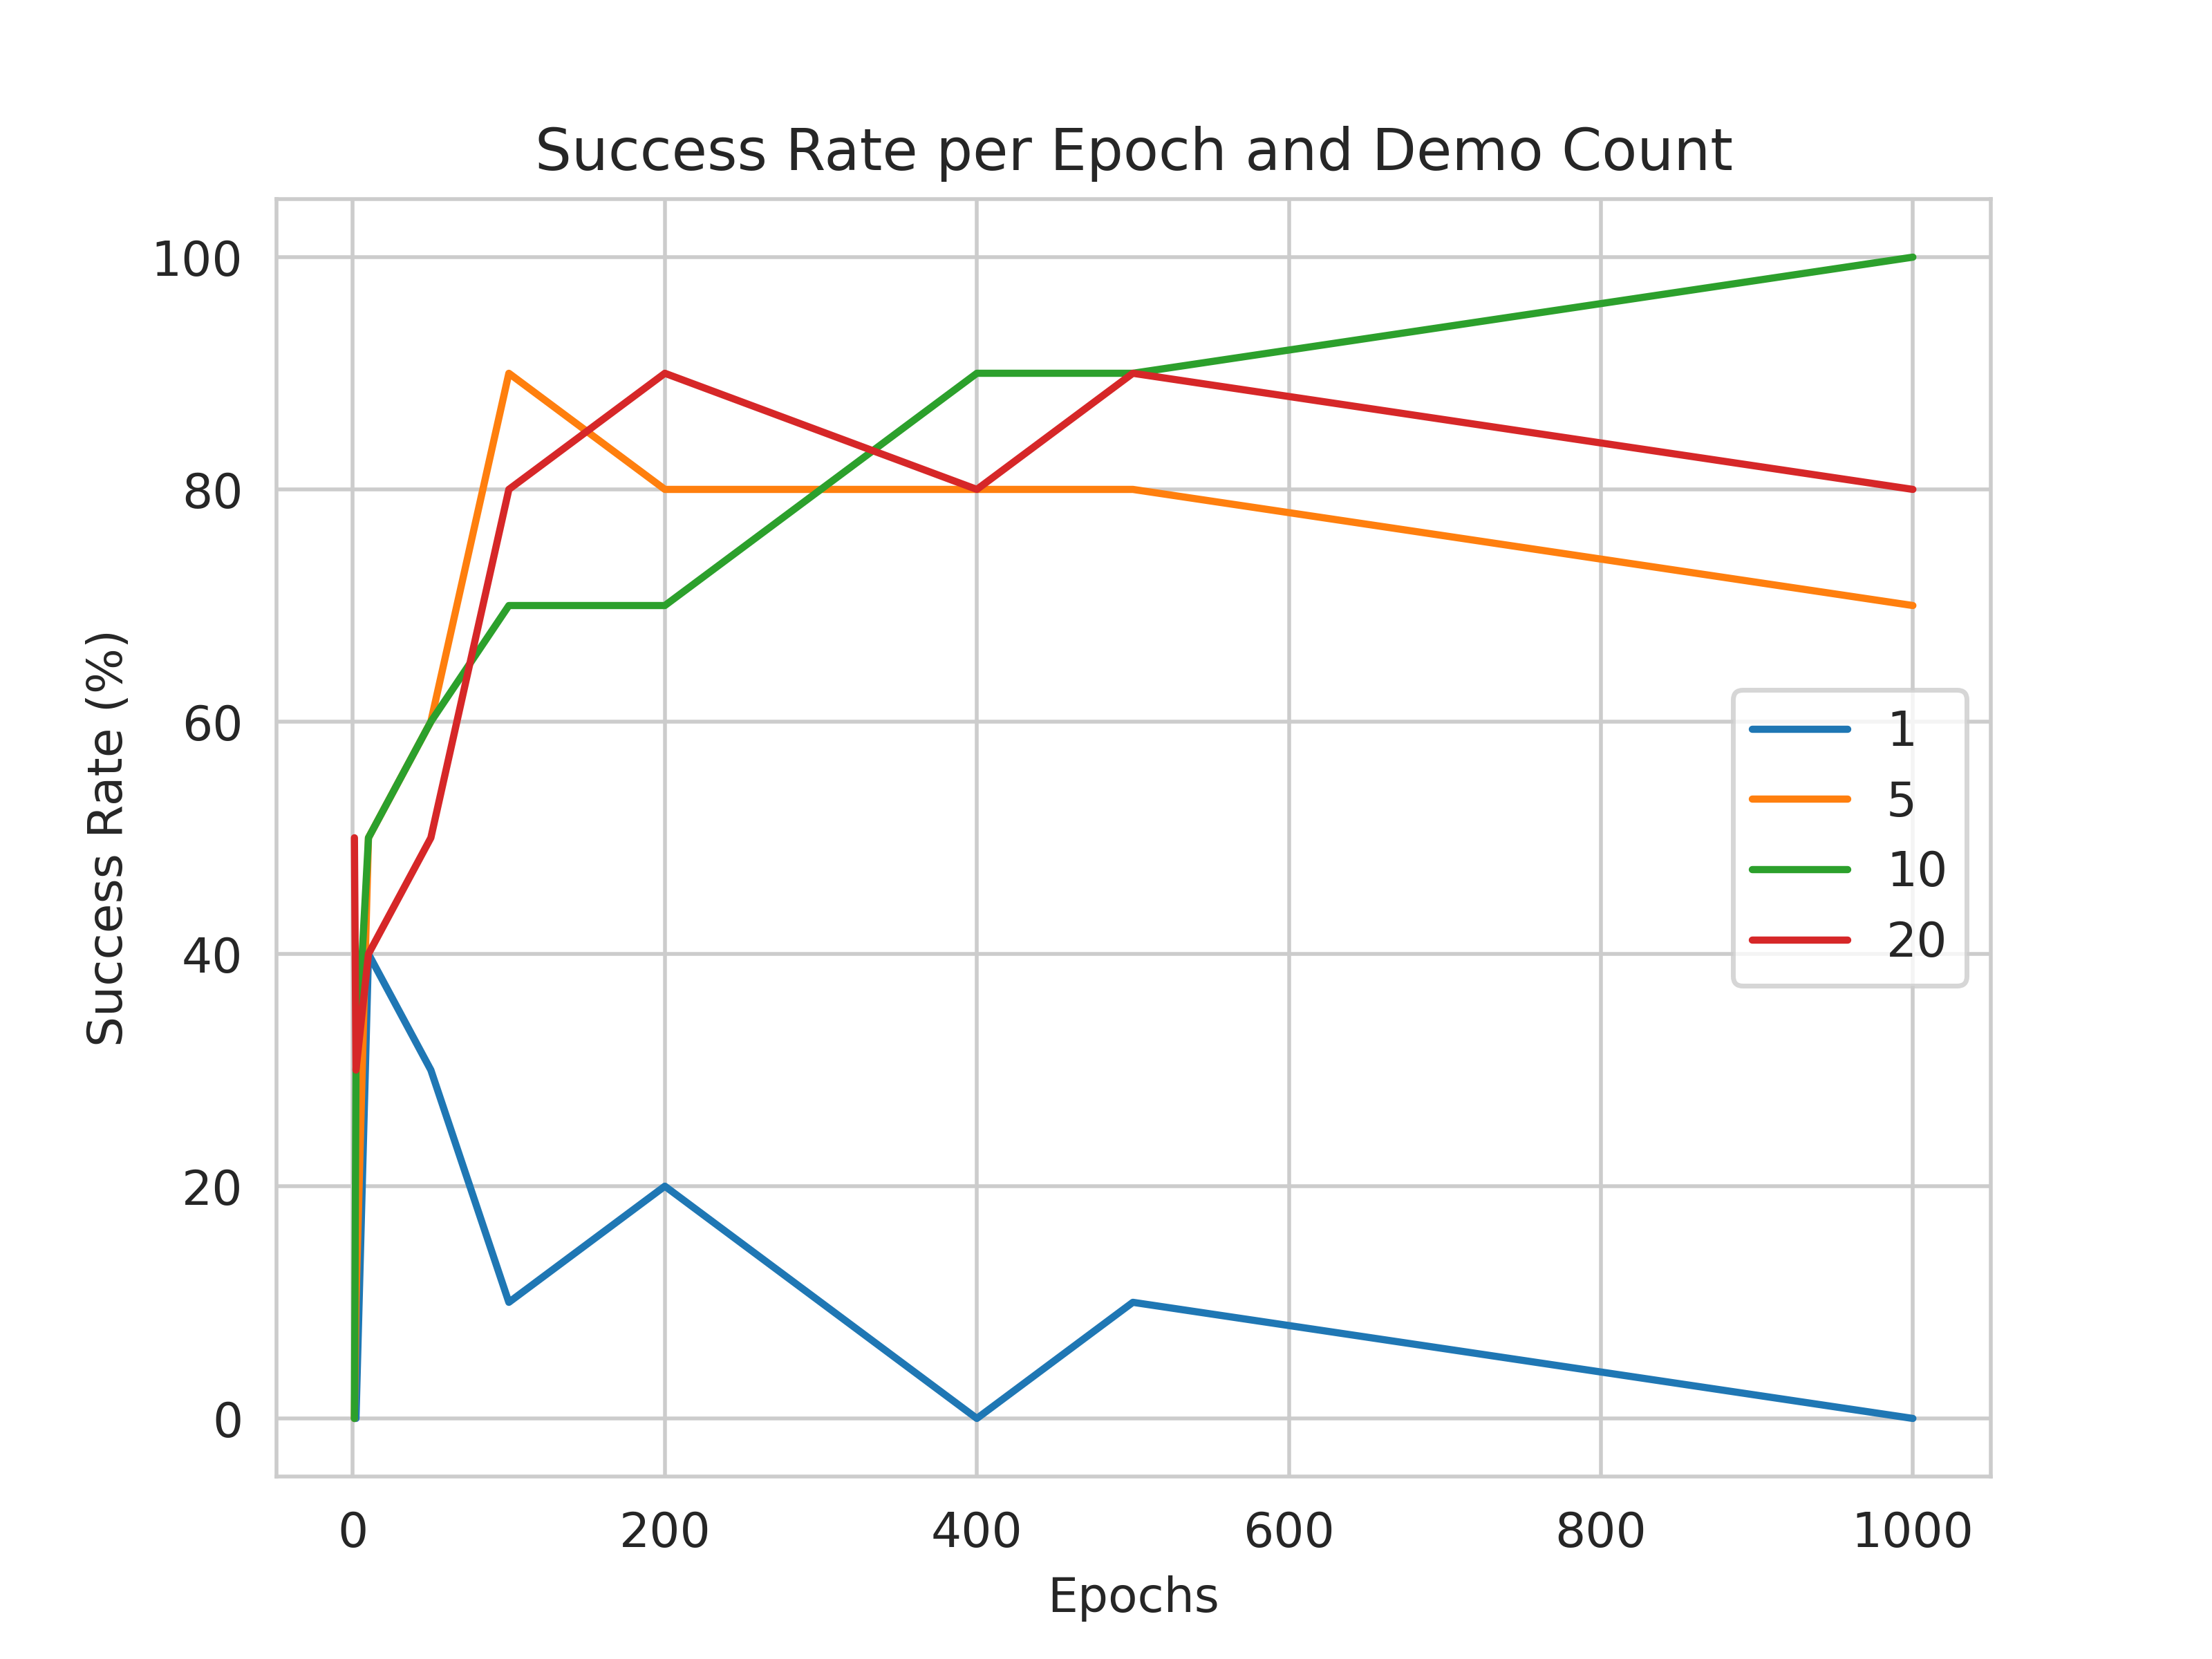
\includegraphics[width=\linewidth]{assets/cam-comb/reach-no-obs/rno_random-success.png}
    \caption{Success Rate (\%) for the $10$ Test Demos}\label{subfig:rno-random-success}
  \end{subfigure}
  \caption{Experiments with randomly placed target}\label{fig:rno-random}
\end{figure}

To run the random tests, shown in Figures \ref{fig:rno-random-dist} and \ref{fig:rno-random-success}, in a comparable manner I reused my set of demos that were created and saved earlier for this task for training. Then a set of 10 demos were randomly generated at the start and after the agent with the specific parameters were trained, I evaluated these policies against the test counterparts.

Looking at graph \ref{subfig:rno-random-dist}, we can see that providing more demonstrations helps the policy generalise better to random locations, where the sweet spots seems to be around 10 demos and around $500$ where the success rate (\ref{subfig:rno-random-success}) is quite high

\subsection{Camera Limitations}
I started this section by limiting the learning to only the wrist mounted camera, which works well for this specific unobscured task. Introducing some of the other RGB cameras, specifically the \textbf{left shoulder} or the \textbf{right shoulder} views, doesn't drastically benefit the performance, other than just the \textbf{right shoulder} RGB, see \ref{fig:rno-random-cams}. Conversely, combining more than one camera seems to be adding to the deficit, as the features being extracted are likely incompatible due to the various view points. 

As the current fusion system does not allow for optimal multi-view feature extraction, using multiple different cameras are not necessarily benefiting the learning and might even be negating its effectiveness due to diluting the features by concatenating incompatible views. \todo[color=green]{ref back to this when needed and improve the policy from now on?} 

A possible explanation as to why the right shoulder camera alone might be increasing success rate is, I think, solely because of its strategic placement compared to the rest of the cameras. 

It is marginally better than wrist, which is likely due to the wrist sometimes observing very similar frames if it happens to initially move away from the target, which can happen when the random target spawn location is out of distribution. Which gets the agent stuck in an unknown state in by these initial erroneous moves. Leading it to not reaching the target. This is not as big an issue with the right shoulder camera, simply due to its larger coverage, and static nature which increases the network potency in repetitive simple movements simply due to the frame of reference never changing.\todo[color=purple]{}. 

To reason why the right shoulder and not the left is simply because of the geometry of the robot. The left camera is more likely to get obstructed by the robot itself due to its top joints being on its left, seen in \ref{subfig:rno-random-ls}. 

So, there is improvement from multiple views, but this task does not really benefit from extra frames of vision. However, this is not to say all tasks will be immune to benefits from extra views. An important part of this project is to understand what is most important for a robot to observe in its given environment and task and how can it optimally leverage this data to solve a task better. And increasingly more complex tasks should benefit from abundance of information.

\begin{figure}[htpb] % htpb allows all placement
  \centering
  \begin{subfigure}{0.3\linewidth}
    \centering
    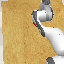
\includegraphics[width=0.5\linewidth]{assets/cam-comb/reach-no-obs/demo1-step30-left_shoulder.png}
    \caption{Left Shoulder}\label{subfig:rno-random-ls}
  \end{subfigure}
  \begin{subfigure}{0.3\linewidth}
    \centering
    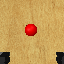
\includegraphics[width=0.5\linewidth]{assets/cam-comb/reach-no-obs/demo1-step30-wrist.png}
    \caption{Wrist}\label{subfig:rno-random-wrist}
  \end{subfigure}
  \begin{subfigure}{0.3\linewidth}
    \centering
    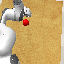
\includegraphics[width=0.5\linewidth]{assets/cam-comb/reach-no-obs/demo1-step30-right_shoulder.png}
    \caption{Right Shoulder}\label{subfig:rno-random-rs}
  \end{subfigure}
  \caption{RGB Views from the first `ReachNoObs\_PlaceRandom' demo (step 30)}\label{fig:rno-random-rgb-views}
\end{figure}

\begin{figure}[htpb] % htpb allows all placement
  \centering
  \begin{subfigure}{0.45\linewidth}
    \centering
    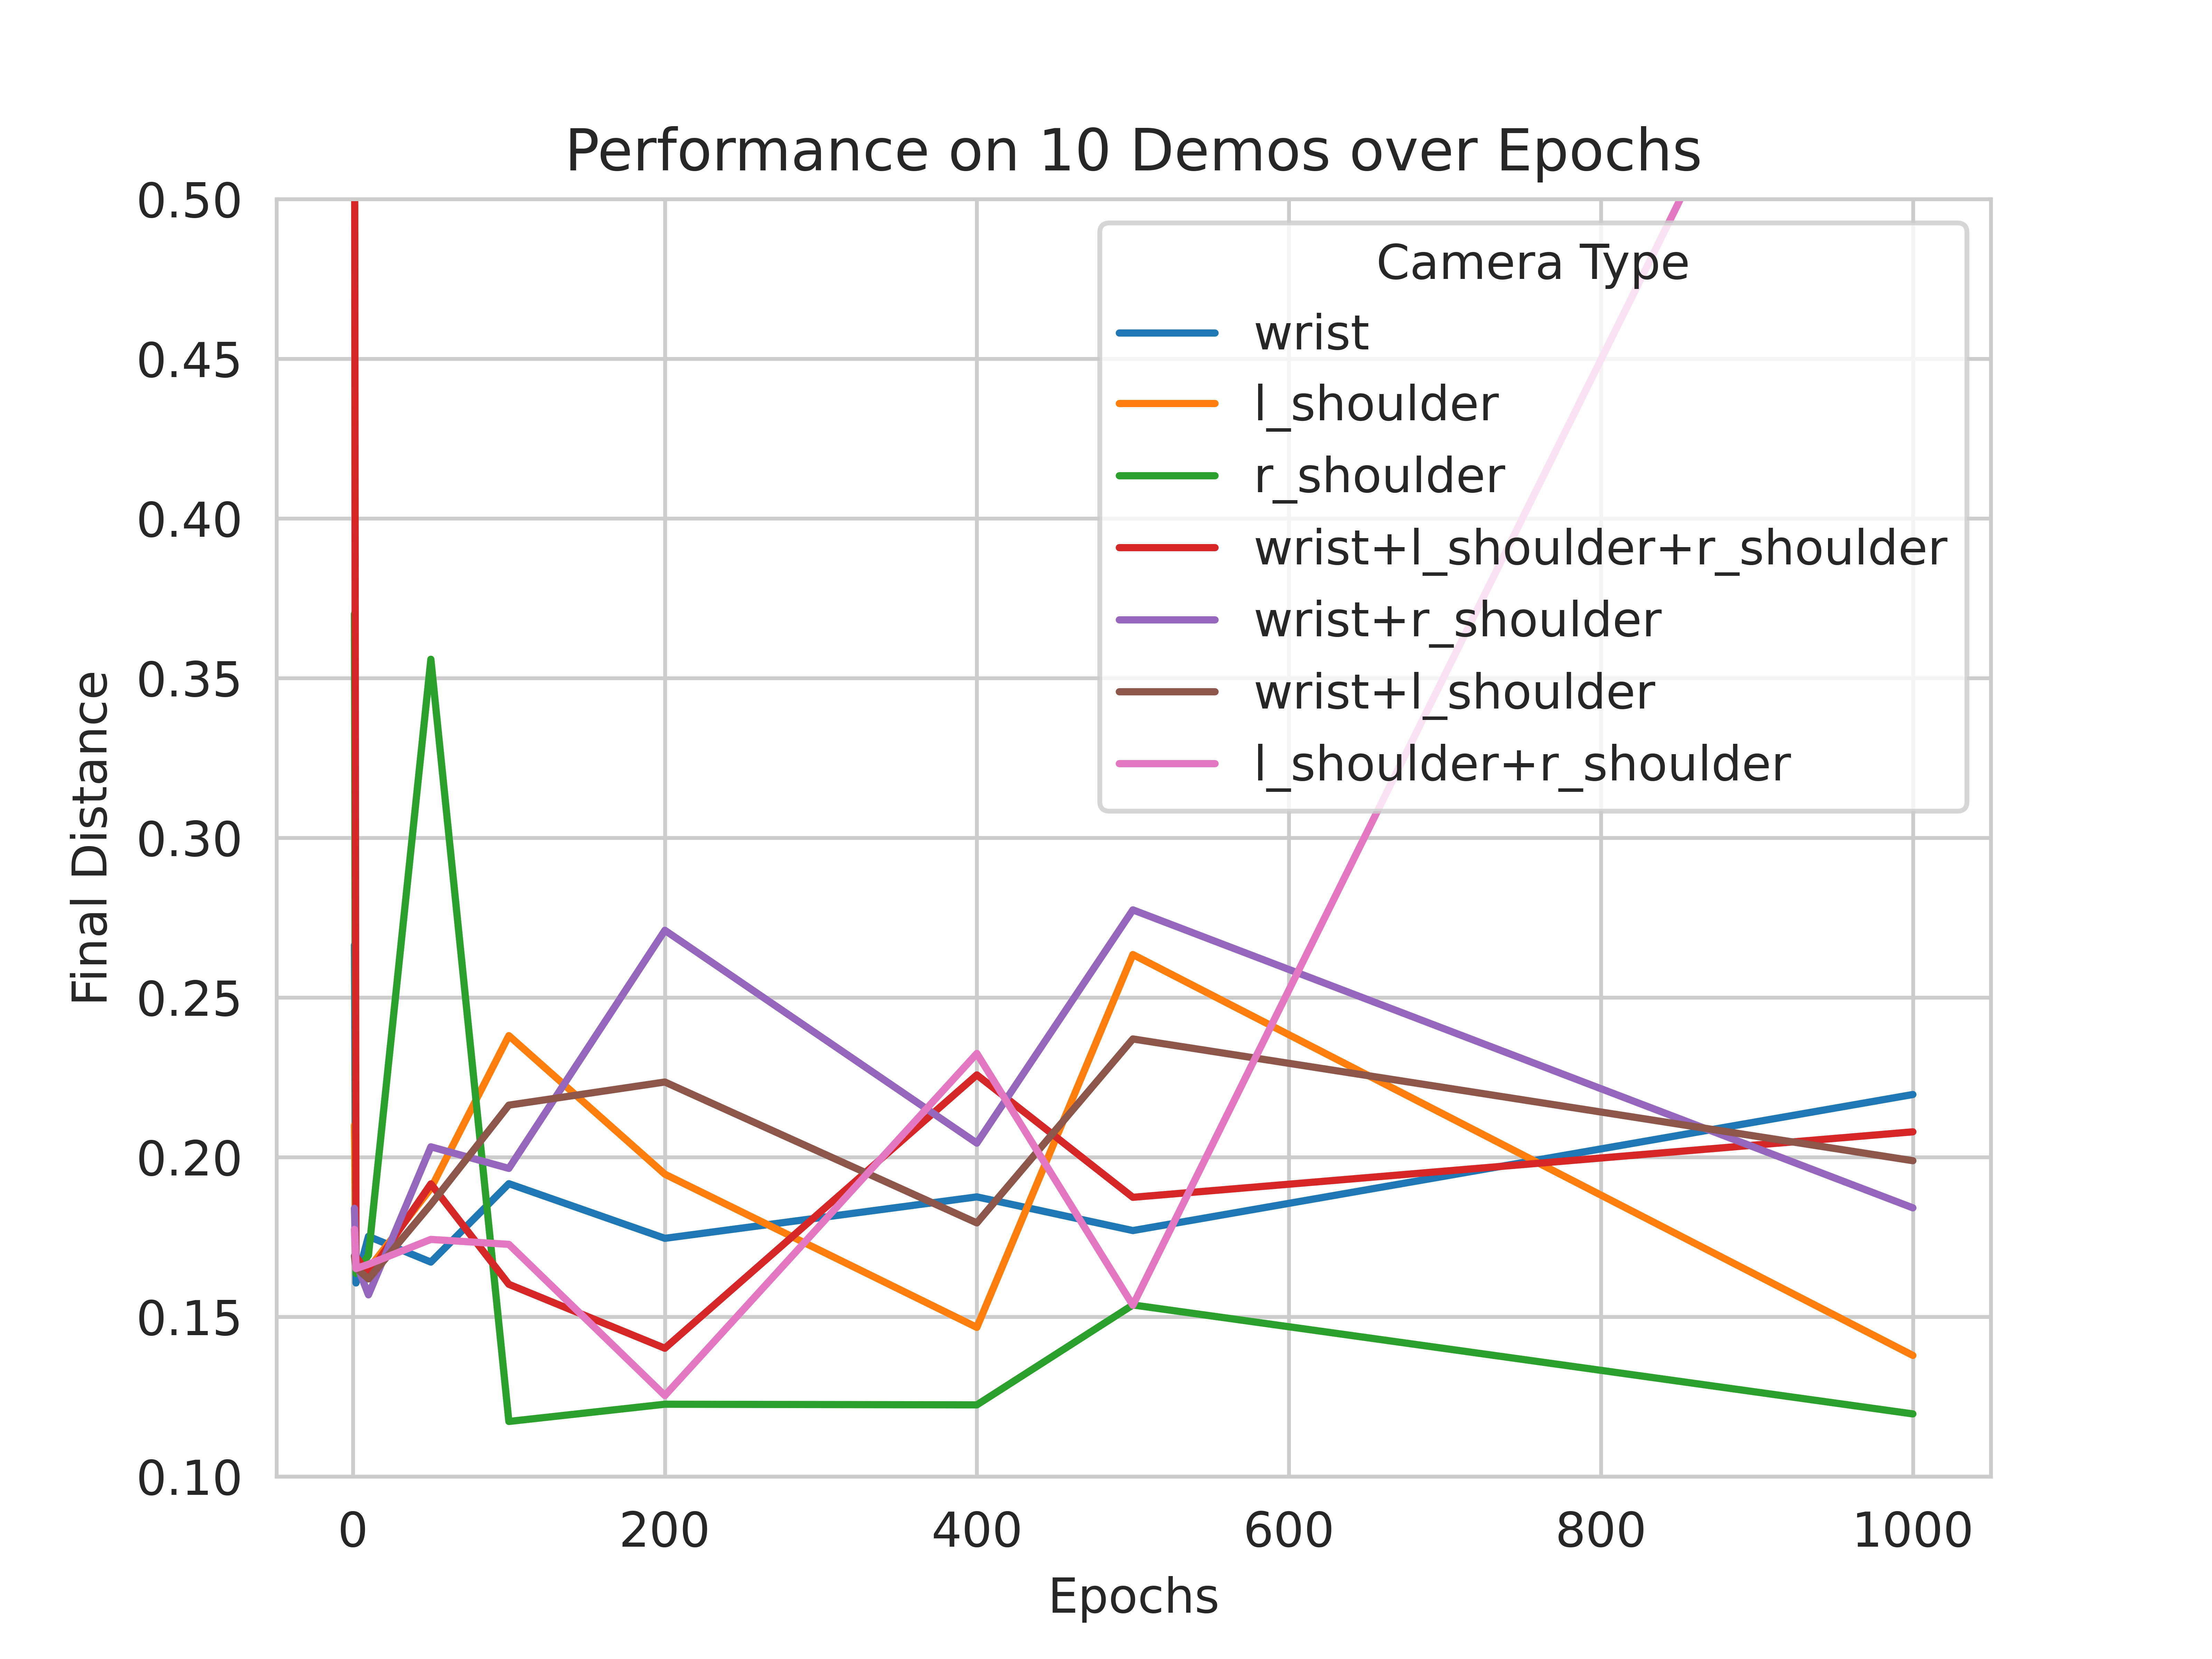
\includegraphics[width=0.7\linewidth]{assets/cam-comb/reach-no-obs/rno_random-cams.png}
    \caption{Average Final Distance to Target}\label{subfig:rno-random-cams-dist}
  \end{subfigure}
  % \hfill
  \begin{subfigure}{0.45\linewidth}
    \centering
    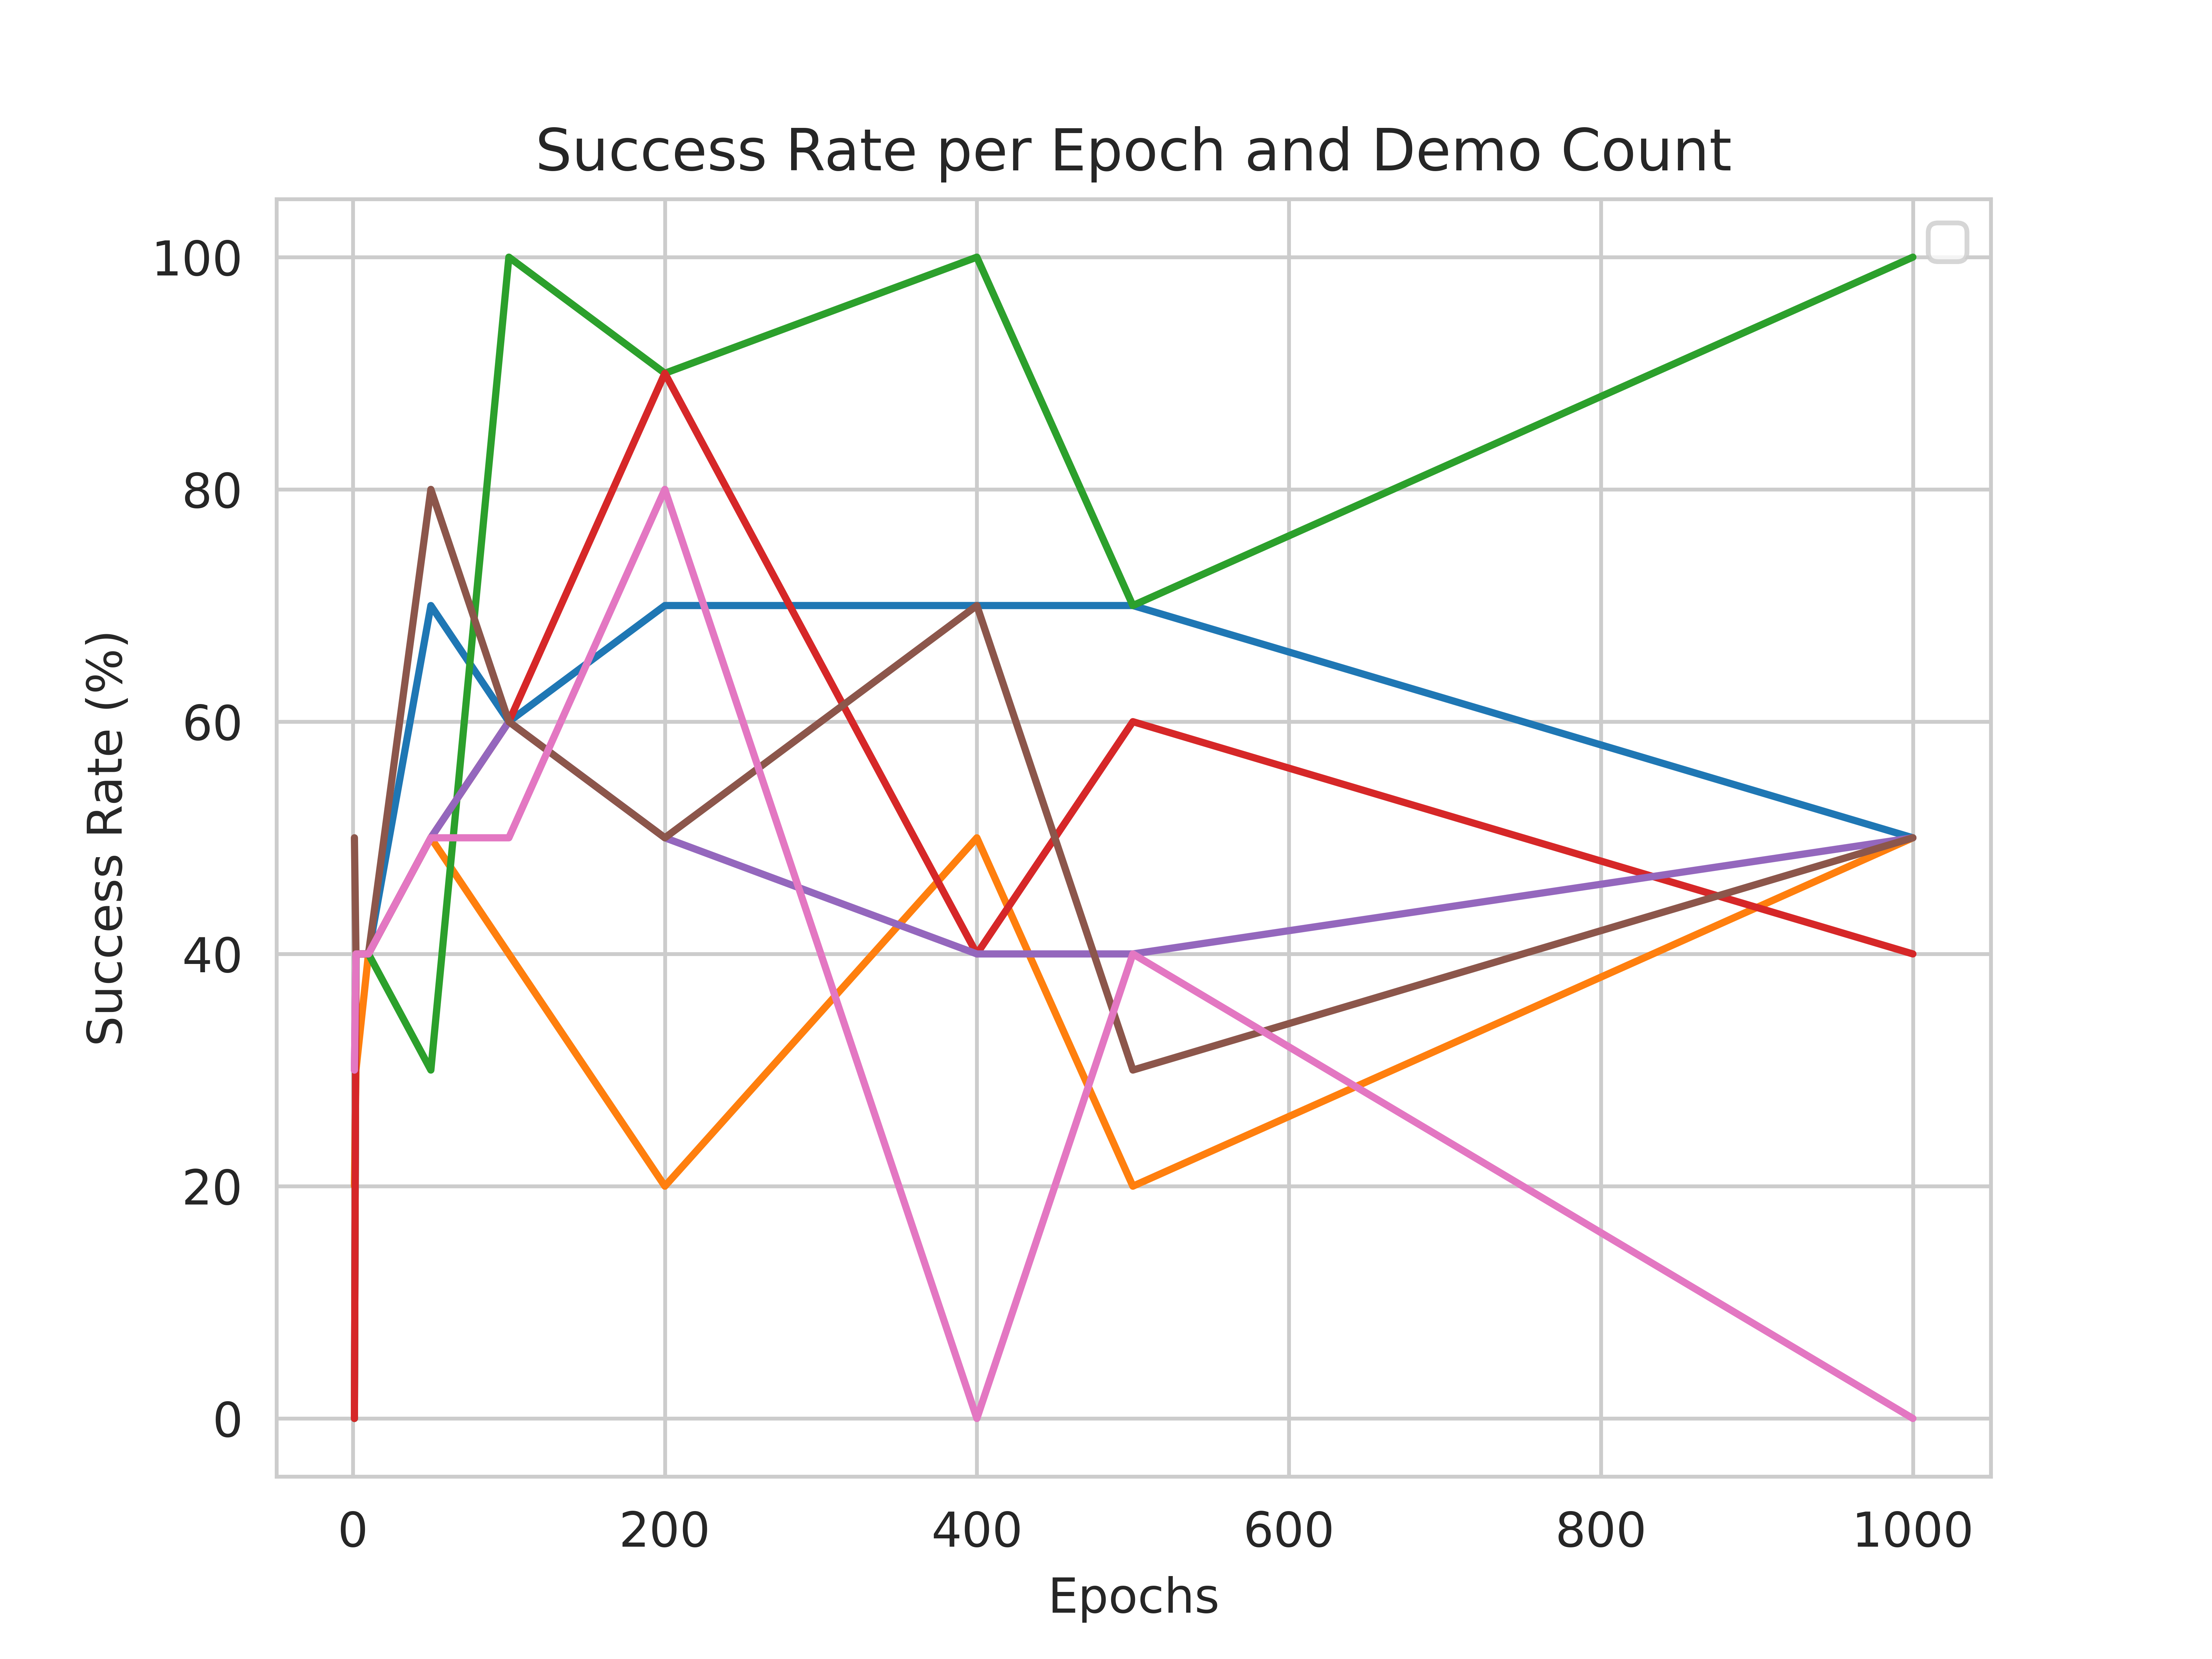
\includegraphics[width=0.7\linewidth]{assets/cam-comb/reach-no-obs/rno_random-cam_success.png}
    \caption{Success Rate (\%) on the $10$ tests}\label{subfig:rno-random-cams-success}
  \end{subfigure}
  \caption{Experimenting with multiple RGB cameras}\label{fig:rno-random-cams}
\end{figure}

\subsection{Increasing the Toy Task Complexity}
Complexity of tasks can be increased in two main ways. (1) Increase the movement or the level of interaction of the task at hand. (2) Introducing non-linearities to the environment to make a scene more challenging to traverse for an agent. I plan to do these mainly by introducing obstacles; which will guide me to understand what an agent needs to understand navigation. Secondly, I want to branch out to a grasping task, to increase the number of items of execution, to evaluate the capability of an agent to use its understanding to complete increasingly more complicated tasks.

